% Bestellingbestuur
\section{Bestellingbestuur}
\subsection{Gebruikersgeval}

\begin{figure}[htbp]
    \centering
    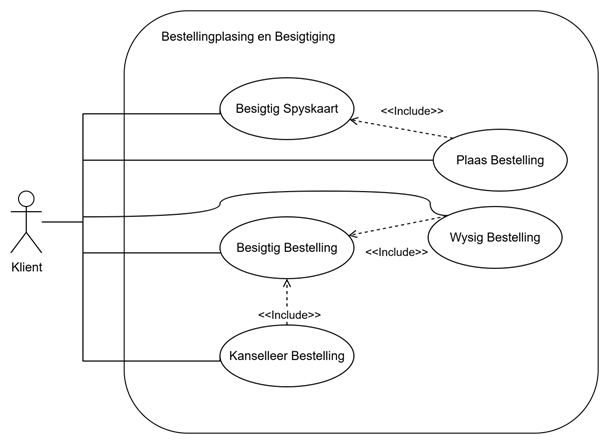
\includegraphics[width=\textwidth]{figures/usecase/orders.png}
    \caption{Gebruikersgeval vir Bestellingbestuur}
    \label{fig:bestellingbestuur_use_case}
\end{figure}

Volgens FREQ-MOB-001 moet gebruikers wat weeklikse spyskaart kan besigtig (\autoref{fig:menu_screen}), en volgens FREQ-MOB-002, FREQ-MOB-003 en FREQ-MOB-004 moet die gebruiker allergie-aanduiders, voedselwaarde en beelde van die maaltye indien beskikbaar getoon word (\autoref{fig:meal_details_screen}). Die stelsel ondersteun slegs die gebruik van 'n rekening waarvan koste gedebiteer word volgens FREQ-MOB-201. Die stelsel moet volgens FREQ-MOB-101 en FREQ-MOB-103 huidige en verlede bestellings toon (\autoref{fig:order_history_screen}).

\subsection{Scenario}

\textbf{Akteurs:} Klient\\
\textbf{Voorvereistes:} Klient is ingeteken\\
\textbf{Prekondisie:} Spyskaart is beskikbaar, gebruiker het genoegsame balans\\
\textbf{Postkondisie:} Bestelling is geplaas, gebruiker se balans word gedebiteer\\
\textbf{Inset:} Gekose Bestelling\\
\textbf{Uitset:} Sukses- of foutboodskap\\
\textbf{Skerms van Toepassing:} 
\begin{itemize}
    \item \autoref{fig:menu_screen} (Spyskaart skerm)
    \item \autoref{fig:orders_screen} (Bestelling skerm)
    \item \autoref{fig:order_success_screen} (Bestelling sukses skerm)
    \item \autoref{fig:order_error_screen} (Bestelling fout skerm)
    \item \autoref{fig:order_history_screen} (Bestelling geskiedenis skerm)
    \item \autoref{fig:meal_details_screen} (Maaltyd besonderhede skerm)
\end{itemize}


\textbf{Hoofvloei:}
\begin{enumerate}
    \item Gebruiker navigeer na spyskaart bladsy (\autoref{fig:menu_screen})
    \item Stelsel toon weeklikse spyskaart met allergie-aanduiders, voedingswaarde en beelde (\autoref{fig:menu_screen}, \autoref{fig:meal_details_screen})
    \item Gebruiker kies maaltyd(e) vir bestelling
    \item Gebruiker spesifiseer hoeveelheid
    \item Stelsel toon bestellingopsomming en totale koste
    \item Stelsel toon gebruiker se huidige rekeningbalans
    \item Gebruiker bevestig bestelling
    \item Stelsel valideer voldoende krediet
    \item Stelsel debiteer gebruiker se rekening
    \item Stelsel skep bestelling rekord
    \item Stelsel toon bestellingbevestiging (\autoref{fig:order_success_screen})
    \item Gebruikersgeval eindig
\end{enumerate}

\textbf{Alternatiewe vloei A1: Besigtig bestellings}
\begin{enumerate}
    \item[1a.] Gebruiker navigeer na "My Bestellings"
    \item Stelsel toon huidige en verlede bestellings
    \item Gebruikersgeval eindig
\end{enumerate}

\textbf{Alternatiewe vloei A2: Wysig bestaande bestelling}
\begin{enumerate}
    \item[1b.] Gebruiker kies bestaande bestelling om te wysig
    \item Stelsel kontroleer of wysiging binne tydsvenster is
    \item Stelsel toon bewerkbare bestelling
    \item Gebruikersgeval eindig
\end{enumerate}

\textbf{Alternatiewe vloei A3: Kanselleer bestelling}
\begin{enumerate}
    \item[1c.] Gebruiker kies bestaande bestelling om te kanselleer
    \item Stelsel kontroleer of kansellasie binne tydsvenster is
    \item Stelsel vra bevestiging vir kansellasie
    \item Gebruiker bevestig kansellasie
    \item Stelsel kanselleer bestelling en krediteer rekening
    \item Stelsel toon kansellasiebevestiging
\end{enumerate}

\textbf{Uitsonderingsvloei E1: Onvoldoende krediet}
\begin{enumerate}
    \item[8a.] Stelsel identifiseer onvoldoende krediet
    \item Stelsel toon "Onvoldoende krediet" fout
    \item Stelsel toon huidige balans en benodigde bedrag
    \item Stelsel bied opsie om admin te kontak
    \item Gebruikersgeval eindig
\end{enumerate}

\textbf{Uitsonderingsvloei E2: Wysiging/kansellasie buite tydsvenster}
\begin{enumerate}
    \item[1d.] Stelsel identifiseer dat tydsvenster verby is
    \item Stelsel toon "Te laat vir wysigings" boodskap
    \item Gebruikersgeval eindig
\end{enumerate}

